\documentclass[10pt, conference, compsocconf]{IEEEtran}
\IEEEoverridecommandlockouts

% Various packages that might be useful
\usepackage[pdftex]{graphicx}
\usepackage{array}
\hyphenation{op-tical net-works semi-conduc-tor}
\usepackage{color}
\usepackage{underscore}
\usepackage{tikz}
\usepackage{algorithm}
\usepackage{comment}
\usepackage{algpseudocode}
\usetikzlibrary{arrows}
\usepackage{flushend}

% Mark this as a draft
%\usepackage{draftwatermark}
%\SetWatermarkText{DRAFT}
%\SetWatermarkScale{1}

\newcommand{\cb}{\textcolor{blue}}
\newcommand{\cred}{\textcolor{red}}
\newcommand{\cg}{\textcolor{green}}


% For algorithm indent
\newcommand{\IndState}[1]{\State\hspace{#1\algorithmicindent}}



\begin{document}

\title{I/O Router Placement and Fine-Grained Routing on Titan to Support Spider II}

\author{\IEEEauthorblockN{Matt Ezell, Sarp Oral, Feiyi Wang, Devesh Tiwari,\\Don Maxwell, Dustin Leverman, and Jason Hill}
\IEEEauthorblockA{Oak Ridge National Laboratory; Oak Ridge, TN\\
\{ezellma,oralhs,fwang2,tiwari,maxwellde,leverman,hilljj\}@ornl.gov}
\and
\IEEEauthorblockN{David Dillow*\thanks{*David Dillow was previously associated with Oak Ridge National Laboratory}}
\IEEEauthorblockA{dave@thedillows.org}
}

\maketitle

\section{Abstract}

The Oak Ridge Leadership Computing Facility (OLCF) introduced the concept of
fine-grained routing in 2008 to improve I/O performance between the Jaguar
supercomputer and Spider, the center-wide Lustre file system. Fine-grained
routing organizes I/O paths to minimize congestion. Jaguar has since been
upgraded to Titan, providing more than a ten-fold improvement in peak
performance. To support the center’s increased computational capacity and I/O
demand, the Spider file system has been replaced with Spider II. Building on
the lessons learned from Spider, an improved method for placing LNET routers
was developed and implemented for Spider II. The fine-grained routing scripts
and configuration have been updated to provide additional optimizations and
better match the system setup. This paper presents a brief history of
fine-grained routing at OLCF, an introduction to the architectures of Titan and
Spider II, methods for placing routers in Titan, and details about the
fine-grained routing configuration.

% vim:textwidth=80:


\begin{IEEEkeywords}
Lustre; Titan; Spider II; Fine-Grained Routing; Router Placement; I/O; ORNL; OLCF
\end{IEEEkeywords}

\section{Background}

Initial FGR for Spider 1

Brief intro to Titan/Atlas Architecture

% vim:textwidth=80:

\section{Placement}

The placement of the I/O routers in a large 3D torus can have an enormous impact
on the traffic patterns and congestion characteristics present in the system.
This is important for maximizing I/O performance as well as minimizing the
interaction between application communication and I/O. Building on the lessons
learned from OLCF's Spider~I implementation of fine-grained routing in 2008, an
improved method for placing LNET routers on Titan was developed and implemented
for Spider~II.

\begin{figure*}[t]
  \begin{center}
    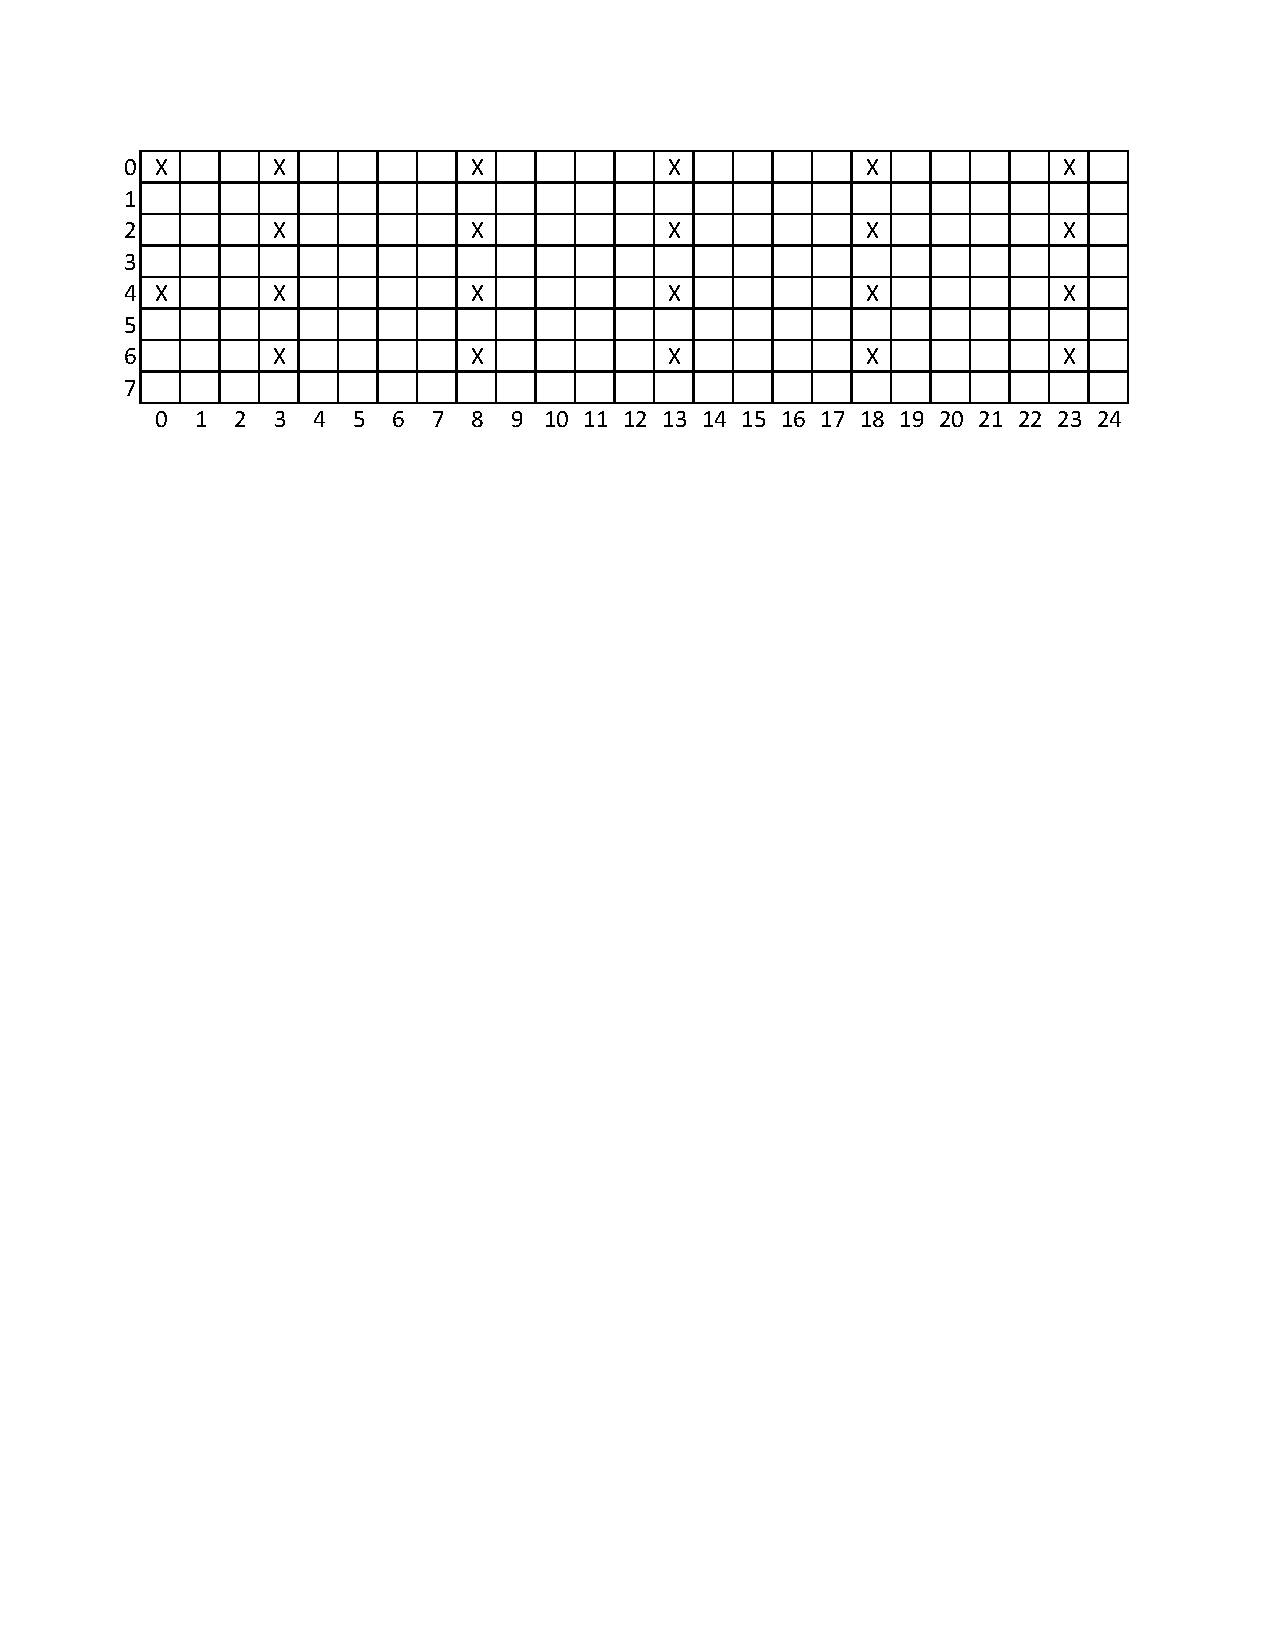
\includegraphics{figures/jaguarplacement}
    \caption{Jaguar Layout}\label{fig:jaglayout}
  \end{center}
\end{figure*}
\begin{figure*}[t]
  \begin{center}
    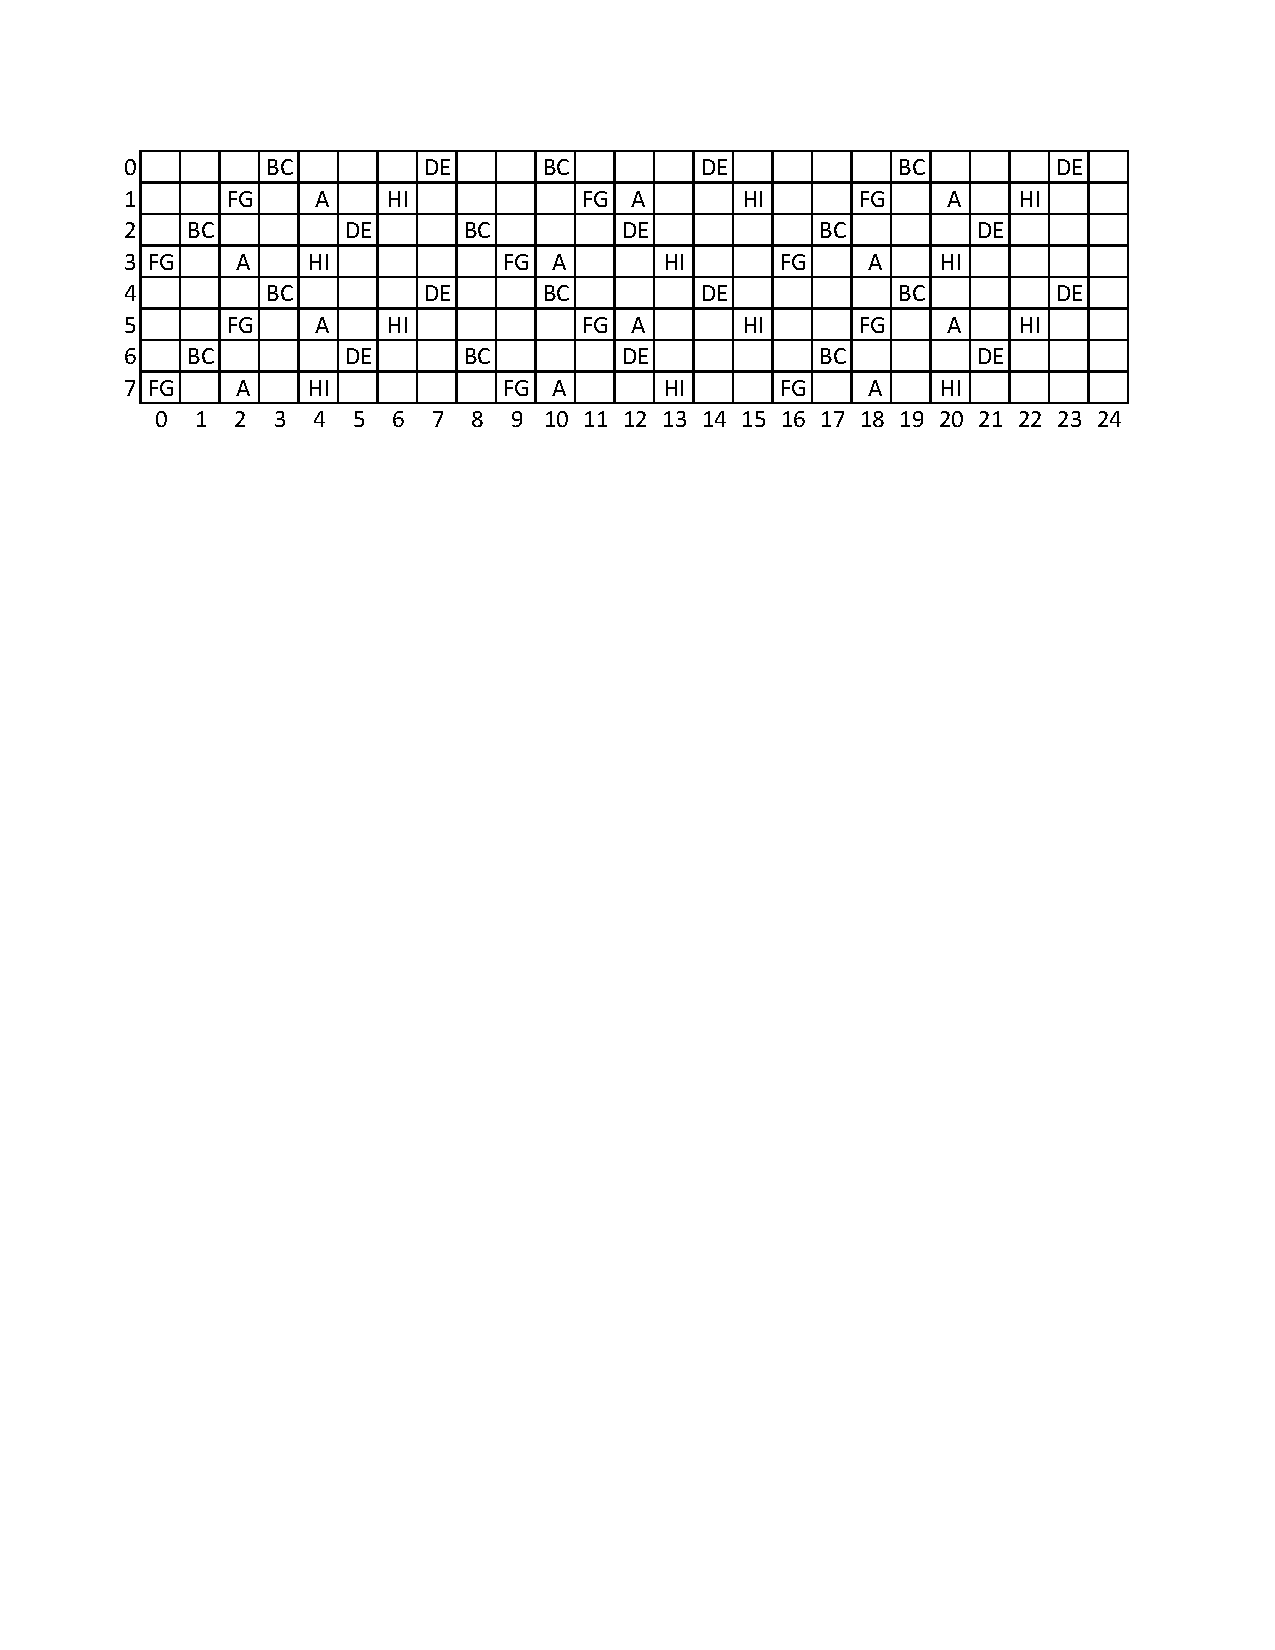
\includegraphics{figures/titanplacement}
    \caption{Titan Layout}\label{fig:titanlayout}
  \end{center}
\end{figure*}

\subsection{Topological Concerns}
\label{sec:topo}

The router placement layout used for Spider~I was designed to distribute the
routers topologically through the machine while also minimizing the number of
cabinets that contained routers (see Figure \ref{fig:jaglayout}). This resulted
in a very regular I/O pattern that was prone to congestion if I/O traffic was
not properly kept localized.

Details about Gemini's architecture and performance characteristics are
available in a paper titled ``Understanding the Impact of Interconnect Failures
on System Operation'' \cite{interconnect} presented at CUG 2013.  Jaguar's
upgrade from Cray's SeaStar interconnect to Gemini significantly changed the
network's characteristics.  Each Gemini supports two nodes, which effectively
halved the Y-dimension length.  Additionally, Y-dimension connections are
comprised of only half the links of X- and Z-dimension connections.  Thus, I/O
traffic should be limited in the Y-dimension due to its reduced relative
bandwidth.  This suggests that routing zones should be ``flattened'' into
``rectangular prisms'' instead of the more traditional cubic zones.

Since Gemini uses dimension-ordered-routing, I/O tends to converge to a single
path as it nears the destination.  Thus, it is important to avoid putting
routers in the same plane.  This can help avoid congestion, but many-to-one
communication patterns in a 3D torus will always suffer from some amount of
congestion.

Minimizing the hop count between clients and routers is essential for providing
high-bandwidth communications with the storage servers.  While Gemini routing
arbitration is locally fair, it is globally unfair.  Packet age and hop-count
are not taken into account when the router selects the next packet to forward.
Figure \ref{fig:geombw} shows an example of this issue.

\begin{figure}[h]
  \centering
    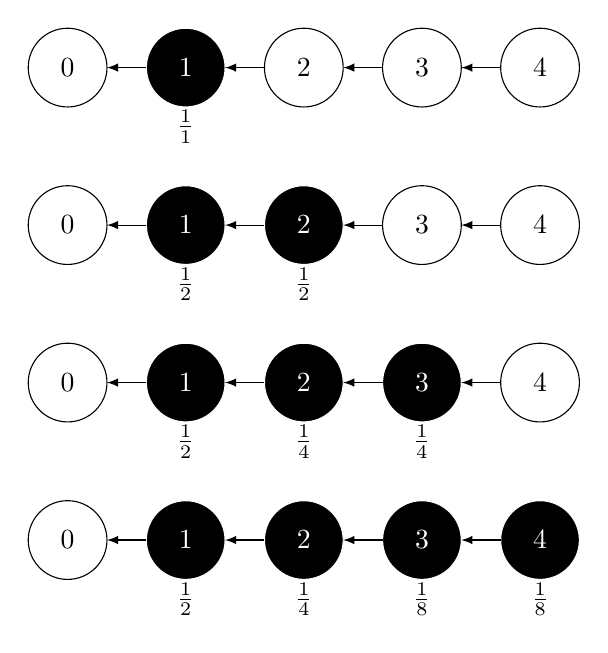
\begin{tikzpicture}
    \def \phase {1}
    \node[draw, circle, minimum height=1cm] at (0,-\phase){$0$};
    \node[draw, circle, minimum height=1cm, color=white, fill=black] at (1.5,-\phase){$1$};
    \node[draw, circle, minimum height=1cm] at (3,-\phase){$2$};
    \node[draw, circle, minimum height=1cm] at (4.5,-\phase){$3$};
    \node[draw, circle, minimum height=1cm] at (6,-\phase){$4$};
    \draw[->, >=latex] (1.0,-\phase) to (0.5,-\phase);
    \draw[->, >=latex] (2.5,-\phase) to (2.0,-\phase);
    \draw[->, >=latex] (4.0,-\phase) to (3.5,-\phase);
    \draw[->, >=latex] (5.5,-\phase) to (5.0,-\phase);
    \node[draw=none] at (1.5,-1.75) {$\frac{1}{1}$};

    \def \phase {3}
    \node[draw, circle, minimum height=1cm] at (0,-\phase){$0$};
    \node[draw, circle, minimum height=1cm, color=white, fill=black] at (1.5,-\phase){$1$};
    \node[draw, circle, minimum height=1cm, color=white, fill=black] at (3,-\phase){$2$};
    \node[draw, circle, minimum height=1cm] at (4.5,-\phase){$3$};
    \node[draw, circle, minimum height=1cm] at (6,-\phase){$4$};
    \draw[->, >=latex] (1.0,-\phase) to (0.5,-\phase);
    \draw[->, >=latex] (2.5,-\phase) to (2.0,-\phase);
    \draw[->, >=latex] (4.0,-\phase) to (3.5,-\phase);
    \draw[->, >=latex] (5.5,-\phase) to (5.0,-\phase);
    \node[draw=none] at (1.5,-3.75) {$\frac{1}{2}$};
    \node[draw=none] at (3,-3.75) {$\frac{1}{2}$};

    \def \phase {5}
    \node[draw, circle, minimum height=1cm] at (0,-\phase){$0$};
    \node[draw, circle, minimum height=1cm, color=white, fill=black] at (1.5,-\phase){$1$};
    \node[draw, circle, minimum height=1cm, color=white, fill=black] at (3,-\phase){$2$};
    \node[draw, circle, minimum height=1cm, color=white, fill=black] at (4.5,-\phase){$3$};
    \node[draw, circle, minimum height=1cm] at (6,-\phase){$4$};
    \draw[->, >=latex] (1.0,-\phase) to (0.5,-\phase);
    \draw[->, >=latex] (2.5,-\phase) to (2.0,-\phase);
    \draw[->, >=latex] (4.0,-\phase) to (3.5,-\phase);
    \draw[->, >=latex] (5.5,-\phase) to (5.0,-\phase);
    \node[draw=none] at (1.5,-5.75) {$\frac{1}{2}$};
    \node[draw=none] at (3,-5.75) {$\frac{1}{4}$};
    \node[draw=none] at (4.5,-5.75) {$\frac{1}{4}$};

    \def \phase {7}
    \node[draw, circle, minimum height=1cm] at (0,-\phase){$0$};
    \node[draw, circle, minimum height=1cm, color=white, fill=black] at (1.5,-\phase){$1$};
    \node[draw, circle, minimum height=1cm, color=white, fill=black] at (3,-\phase){$2$};
    \node[draw, circle, minimum height=1cm, color=white, fill=black] at (4.5,-\phase){$3$};
    \node[draw, circle, minimum height=1cm, color=white, fill=black] at (6,-\phase){$4$};
    \draw[->, >=latex] (1.0,-\phase) to (0.5,-\phase);
    \draw[->, >=latex] (2.5,-\phase) to (2.0,-\phase);
    \draw[->, >=latex] (4.0,-\phase) to (3.5,-\phase);
    \draw[->, >=latex] (5.5,-\phase) to (5.0,-\phase);
    \node[draw=none] at (1.5,-7.75) {$\frac{1}{2}$};
    \node[draw=none] at (3,-7.75) {$\frac{1}{4}$};
    \node[draw=none] at (4.5,-7.75) {$\frac{1}{8}$};
    \node[draw=none] at (6,-7.75) {$\frac{1}{8}$};
  \end{tikzpicture}


  \caption{Geometric Bandwidth Reductions}\label{fig:geombw}
\end{figure}

Node 0 can be considered an I/O router while the others are acting as clients
attempting to send data to the router.  When only node 0 is communicating, it
is able to achieve 100\% of the bandwidth across the link.  Once node 2 starts
communicating, the router attached to node 1 accepts half the bandwidth from
node 1 and half from node 2.  Effectively, the bandwidth is shared between the
nodes.  When node 3 begins communicating, the router attached to node 2 fairly
arbitrates traffic between nodes 2 and 3.  Since that router only has half of
the global bandwith, nodes 2 and 3 each only get one quarter of the total
bandwith to the router.  When node 4 begins communicating, the problem becomes
even more obvious.  The router attached to node 3 fairly arbitrates traffic
between nodes 3 and 4, but it can only grant one eighth of the total bandwidth
to each.

As these chains get longer and longer, the bandwidth available to the ``last''
node can become abysmal.

\subsection{Physical Constraints}


The following physical constraints and goals were kept in mind while
determining an optimal placement algorithm:

\begin{description}
  \item[Topological Concerns] \hfill \\
    Routers must be placed to optimize for the topological concerns mentioned
    in Section \ref{sec:topo}.
  \item[Minimize Cabinet Count] \hfill \\
    Each cabinet that contains a router module requires a hole to be drilled in
    the floor to accomodate the cables.
  \item[Cable Length] \hfill \\
    Shorter cables are cheaper and easier to manage in the data center.
  \item[Partitionability] \hfill \\
    Occasionally, Titan's 3D torus must be partitioned to facilitate extended
    maintenance activites or testing.  During this situation, it is important to
    ensure full routability to boot from both ``ends'' of the machine.  A boot
    node is located in physical columns 0 and 24 (topological columns 0 and 13).
    Thus, routers should be located in a way that minimizes the number of
    columns required to access the entire file system.
\end{description}

\subsection{Implementation}

In the Cray~XK architecture, each service module contains four service nodes.
Since each service module displaces a compute module, it is important to
utilize each node.  Ideally, the LNET routers would exist on the same module as
less bandwidth-intensive nodes (such as a login nodes).  This is unfortunately
impossible due to the sheer number of routers required to achieve sufficient
bandwidth.

Having 4 routers on a module matches nicely with the 4 rows of Spider~II.  The
nodes on a given module will connect to a switch in each of the 4 rows of
Spider~II.  There is a ``swizzle'' to spread Gemini load.

As part of the Spider~II upgrade, the number of LNET routers on Titan was
doubled to 440 nodes and each router was equipped with an IB FDR HCA with 16
PCI-E lanes running at Gen-2.

% vim:textwidth=80:

\section{Fine-Grained Routing}

%\cb{Devesh: Currently holding lock on this section.: not any more}

The first step towards achieving higher performance is to place LNET routers equidistant from each other as much as possible,
subject to physical constraints and other boundary conditions. This ensures that LNET routers are distributed across the machine
and are not segregated in a particular zone. The second key step is to pair clients with their closet possible LNET router. This 
section discusses the algorithm that pairs a client with the closet possible LNET router to minimize hop counts and congestion.

Recall that there are a total 440 LNET routers where only 432 routers are used for file I/O and rest 8 are used for meta data I/O.
Four LNET routers together form a router module, resulting in a total of 108 router modules in the system. These 108 router modules 
are divided into 9 groups. Each group is further divided into 4 sub-groups. Each sub-group consists of 3 router modules. Therefore, each 
group consists of 12 router modules.

%\cb{Devesh: need to describe why 4 and 9? it is because of corresponding rows and columns of DDN storage racks?}

Algorithm~\ref{alg:fgr} describes how a client chooses the closet router module within the assigned group. We note that
the client to group pairing is decided using a fixed arrangement. Before we describe the algorithm in detail, we first
describe how a particular router module is denoted in our algorithm depending on its association with a particular group and sub-group. The 
$i^{th}$ router module in the $G^{th}$ group and $S^{th}$ sub-group is denoted as $R^G_{i}(S)$. Based on 
our previous discussion, we can infer that $G$, $S$ and $i$ will have following respective ranges: ($1, \dots, 9$), ($1, \dots, 4$), 
and ($1, \dots, 3$).

The algorithm takes two input parameters: first, coordinates of the client ($C$) and second, the group it belongs to ($R^G$). The 
algorithm returns the coordinates of three routers assigned to the input client ($C$), one primary and two backup routers. 

Our fine-grained algorithm consists of two steps. The first step (line~\ref{first:begin}--\ref{first:end}) is to choose the sub-group whose 
Y-coordinates fall within the close range of Y-coordinates of the input client, $C$. This is because the bandwidth in the Y-direction is limited
compared to other directions, as discussed earlier. Therefore, it is desirable to minimize the traffic in that direction first. 

Once the sub-group is selected, the second step (line~\ref{second:begin}--\ref{second:end}) is to return assigned routers from this sub-group.
As mentioned earlier, each sub-group consists of 3 routers and the algorithm returns a vector of 3 routers. So, all three of them are 
returned, but the one with the lowest distance in X-dimension is assigned as the primary router to minimize the hops and avoid congestion 
in that direction. We note that the X-direction crosses cabinet boundaries, therefore it more desirable to minimize the hops in that 
direction compared to the Z-direction that run within a cabinet in vertical direction.


\begin{algorithm}
\caption{Fine-grained routing algorithm}
\label{alg:fgr}
\begin{algorithmic}[1]
\Procedure {Route Selection Algorithm }{$R^G$, $C$} \\ 
%\hrulefill
\State Divide $R^G$ into 4 sub-groups: $R^G(1)$ \ldots $R^G(4)$.

\ForAll{sub-groups $R^G(i)$} \Comment{$i$ ranges 1 to 4}
\label{first:begin}
    \State $C[y]$ $\leftarrow$ y coordinate of $C$
    \State $R^G_{1}(i)$ $\leftarrow$ first router module in the $i^{th}$ sub-group
    \State $R^G_{1}(i)[y]$ $\leftarrow$ y coordinate of $R^G_{i}(S)$
    \If{ ($C[y] == R^G_{1}(i)[y]-1$) 
    \\ \hspace{\algorithmicindent} \hspace{\algorithmicindent}   or ($C[y] == R^G_{1}(i)[y]$)
    \\ \hspace{\algorithmicindent} \hspace{\algorithmicindent}   or ($C[y] == R^G_{1}(i)[y] + 1$) 
    \\ \hspace{\algorithmicindent} \hspace{\algorithmicindent}   or ($C[y] == R^G_{1}(i)[y] + 2$)}
    \State break with sub-group $i$ selected
    \EndIf
\EndFor
\label{first:end}

\\ 

\State $i$ $\leftarrow$ index of selected sub-group
\label{second:begin}
\State $r_1, r_2, r_3$ $\leftarrow$ first, second, and third router module 
\State \hspace{\algorithmicindent} selected sub-group $i$

\State $d_{min}$ $\leftarrow$ $\infty$ 
\State $Index_{primary}$ $\leftarrow$ $\infty$

\\

\For{$j$ in $1, \dots, 3$}
    \State $d_{current}$ $\leftarrow$ dist($C[x], r_j[x]$) \Comment{distance along $X$ dimension}
        \If{$d_{current}$ $<$ $d_{min}$}
        \State $Index_{primary}$ $\leftarrow$ $j$
        \EndIf

%    \State primary router module $\leftarrow$ min($d_min$)
%    \State backup router modules $\leftarrow$ 
%    \IndState{0} two other modules in the sub-group 
\EndFor

    \State primary router module $\leftarrow$ $R^G_{Index_{primary}}(i)$
    \State backup router modules $\leftarrow$ 
    \IndState{0} two other modules in the $i^{th}$ sub-group

    \Return $<$primary and backup router modules$>$ \\ 

\label{second:end}

\EndProcedure
\\
%\hrulefill
\end{algorithmic}
\end{algorithm}

\begin{comment}
With router placement in place, we now face the question that, how does each
client select which router to minimize communication hops as well as to avoid
congestion. This section provides an overview on route selection process and
algorithms. Routers are divided into 9 groups, with each group containing 12
router modules. We denote a router group with a superscript, and a router
module in that group with a subscript. For example, the first module in a
router group $A$ is denoted as $R^A_1$ so on and so forth. The following
algorithm describe the core idea of selection process. The input is a given
router group and client ID, the output is a triple: primary router and two back
up routers.
\end{comment}

%Zones in the network

%Return traffic routing

%FGR scripts

% vim:textwidth=80:

% vim:textwidth=80:
\section{Issues}

The I/O router placement attempts to address the issue of traffic routing and
imbalance at system level. The route selection algorithm aims to minimize hops
and mitigate contention between the compute clients and I/O routers. However,
two issues remain evident. First of which is, this mitigation and balancing
strategy extends only to I/O routers, it is \emph{not} a end-to-end complete
solution. Secondly, the benefits of such placement strategy can only be
full realized when the whole system is under the control such that only
selected clients perform I/O on pre-determined targets. 

Due to aforementioned limitations, we have been working on a end-to-end,
balanced data placement strategy to complement the backend fine grain routing
algorithm. The primary goal is to extend the balancing beyond I/O routers and
into the final destination. This work remains a work in progress though.




\section{Conclusion}

The evolution of compute platforms at Oak Ridge National Laboratory has
necessitated unique designs for the storage systems that support them.  Lessons
learned from the deployment and operation of the Spider~I file system led to
the development of fine-grained routing to improve throughput and minimize
congestion.  The Spider~II system was designed and built with fine-grained
routing as a core component.  To support this new file system, the quantity of
I/O routers in Titan was increased and they were carefully placed to minimize
congestion.  A new fine-grained routing mechanism was created that was tailored
specifically to the two systems.

% vim:textwidth=80:

\section{Acknowledgement}

This research used resources of the Oak Ridge Leadership Computing Facility,
located in the National Center for Computational Sciences at Oak Ridge National
Laboratory, which is supported by the Office of Science of the Department of
Energy under Contract DE-AC05-00OR22725.

Notice: This manuscript has been authored by UT-Battelle, LLC, under Contract
No. DE-AC05-00OR22725 with the U.S. Department of Energy. The United States
Government retains and the publisher, by accepting the article for publication,
acknowledges that the United States Government retains a non-exclusive,
paid-up, irrevocable, world-wide license to publish or reproduce the published
form of this manuscript, or allow others to do so, for United States Government
purposes.

% vim:textwidth=80:



% references section
\bibliographystyle{IEEEtran}
\bibliography{cug14-fgr}
%\bibliography{IEEEabrv,cug14-fgr}

% that's all folks
\end{document}


